\section{QT Demodulation}

\begin{figure}
    \centering
    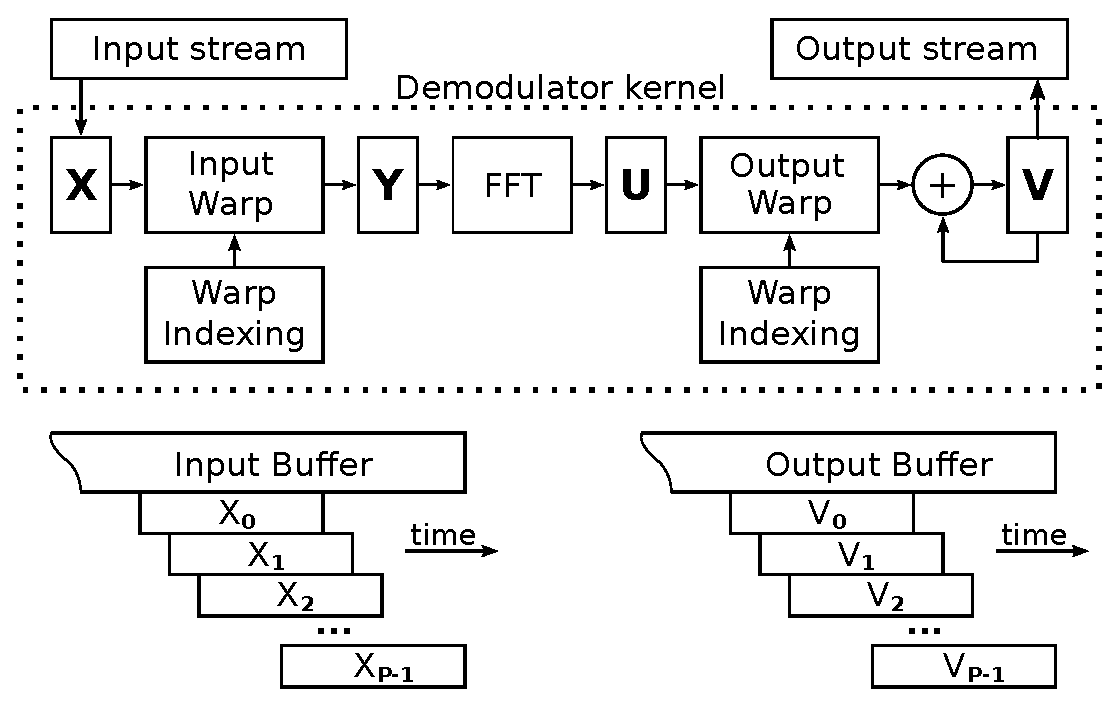
\includegraphics[width=0.95\linewidth]{../source/demod_e}
    \caption[Quantum to Relative Time Demodulation]{Demodulation data flow}
    \label{fig:demod}
\end{figure}

Due to the low I/O bandwidth, the algorithm lends itself to parallelism without
the complexity of high-speed signaling or memory management.
A low-cost ASIC would be feasible for consumer applications.

The mathematics of signal conversion, besides FFT, is mainly College Algebra.
The algorithm can be coded by a typical programmer or engineer with some help
from the following derivations.

%%%%%%%%%%%%%%%%%%%%%%%%%%%%%%%%%%%%%%%%%%%%%%%%%%%%%%%%%%%%%%%%%%%%%%%%%%%%%%%%
\subsection{Input Warping}

The downsampling process of Fig.~\ref{fig:demod} translates the sample pitch of
X to the sample pitch of Y using an exponential sweep.
In the industry, this is known as exponential time-warping.

An exponential chirp sweeps from $f_0$ to $f_1$ in a time T.
M points of X get mapped onto N points of Y, where $M < N$.
Regardless of the sign of $R$, the input warp shifts the corresponding chirp
to the lesser of $f_0$ and $f_1$. The highest frequency component in the input
is $frac{F_S}{2} \cdot frac{1}{1 + |R|}$. Input interpolation produces noise
artifacts, as you would expect. 
As it turns out, they get spread broadly across the spectrum above the region of
interest. Those FFT outputs are ignored.
That's fabulous news, because it removes any motivation for much more
compute-intensive resampling algorithms. Warping may be kept simple and fast.

Let R be a scaled version of $\omega$ for use in the exponential warp and
$\alpha$ the X input sample rate in samples per second.
Given a particular R and N, M and $\omega$ may be calculated.
Let $\epsilon = (f_1/f_0)^{1/T}$. The frequency with respect to time is:
\begin{equation}  \label{eq:fvsf0}
f = f_0 \cdot e^{\epsilon t}
\end{equation}

\subsubsection{Math}

The period of the incoming chirp changes exponentially with index n of $X[n]$.
Let $y = e^{|R|/N}$ be the pitch that accumulates along X.
It has units of ``e's per sample''.
As a scale factor, let $\omega = \frac{\alpha R}{N}$,
in units of ``e's per second'' e/s.
M is the number of input samples warping onto N points.
To time-warp the input, let N be a sum of M segments whose size starts at 1 and
get compressed exponentially. 
The calculation of M starts with a geometric progression in Eq. \ref{eq:M_N0}.

\begin{equation}  \label{eq:M_N0}
N = \sum_{k=1}^{M} e^{-|R| \cdot (k-1)/N} = \frac{1 - e^{-|R| \cdot M/N}}{1 - e^{-|R|/N}}
\end{equation}

\begin{equation}  \label{eq:M_N}
M = \frac{-N}{|R|} \cdot\ ln\left( 1 - N(1-e^{-|R|/N}) \right)
\end{equation}

Re-sampling is done on N points (of Y) at a time where the respective indices of
X and Y are $\delta$ and i.
X is swept from X[0] to X[M-1] or X[M-1] to X[0].

Interpolating from a fractional X index can be done by cubic interpolation
using a Catmull-Rom spline. 
Linear interpolation may be used although it's a little noisier.
The noise extra noise might not make a difference.
Cubic interpolation is a very useful and interesting technique in computing,
so let's touch on that anyway.

Given four points $y_0, y_1, y_2, y_3$, a cubic polynomial describes the curve
passing through all four points, whose slope matches up between adjacent segments.
With $x$ ranging from 0 to 1 indexing the point on $[y_1, y_2]$.

\begin{equation}  \label{eq:cubic}
f = a_0 \cdot x^3 + a_1 \cdot x^2 + a_2 \cdot x + a_3
\end{equation}

\begin{gather*} 
a_0 = -0.5y_0 + 1.5y_1 - 1.5y_2 + 0.5y_3;\\
a_1 = y_0 - 2.5y_1 + 2y_2 - 0.5y_3;\\
a_2 = -0.5y_0 + 0.5y_2;\\
a_3 = y_1;
\end{gather*}

The time span is from 0 to i/N where i sweeps from 0 to N-1 and N is the number
of samples.
Let $\lambda$ be the sample pitch of X.
It will increase or decrease exponentially and should have a maximum value of 1.

This causes a chirp of matching R to be re-sampled to the upper frequency
(either $f_0$ or $f_1$ depending on the sign of R).
Given output index i, input sample index $\delta(i)$ is the accumulated sum of
$\lambda(i)$ when $\lambda$ starts at 1.0 and increases exponentially
or starts at $e^{M \cdot R/N}$ and decreases exponentially.
The exponential sweep can be implemented with a multiplier.
For each step:
\begin{equation}  \label{eq:lambda}
\lambda = \lambda + (\lambda\cdot\Lambda)
\end{equation}

The initial value of $\lambda$ is $e^{M \cdot R/N}$ when $R>0$; otherwise, it's 1.
The ``repeated multiply'' approach to exponential sweep is nearly base $e$,
but it needs a small correction factor to hit $e$.
Setting $e^R = (1 + \Lambda)^N$,
\begin{equation}  \label{eq:lambdaApprox}
\Lambda = e^{R/N} - 1
\end{equation}

A sample C implemention of the warp transform using cubic interpolation is:

\begin{verbatim}
void Warp(
  float* out,        // output stream
  float* in,         // input stream
  int length,        // points in output stream
  double delta,      // starting input index, 0 to 1
  double pitch,      // exponential input sample pitch
  double lambda,     // rate of change of pitch
  double amplitude,  // starting amplitude
  double fcomp)      // decay rate of amplitude
{
  float y0 = *in++;
  float y1 = *in++;
  float y2 = *in++;
  float y3 = *in++;
  // coefficients for first y1-y2 segment of the curve
  float a0 = -0.5 * y0 + 1.5 * y1 - 1.5 * y2 + 0.5 * y3;
  float a1 = y0 - 2.5 * y1 + 2.0 * y2 - 0.5 * y3;
  float a2 = -0.5 * y0 + 0.5 * y2;
  float a3 = y1;
  for (int i = 0; i < length; i++) {
    float x = delta; // between 0 and 1 on y1-y2 path
    float sum = x * (x * (x * a0 + a1) + a2) + a3;
    *out++ = sum * amplitude; // deemphasize low end
    delta += pitch;
    if (delta >= 1.0) {
      delta -= 1.0;
      pitch += pitch * lambda;
      amplitude += amplitude * fcomp;
      y0 = y1;       // stepped into the next segment
      y1 = y2;
      y2 = y3;
      y3 = *in++;
      a0 = -0.5 * y0 + 1.5 * y1 - 1.5 * y2 + 0.5 * y3;
      a1 = y0 - 2.5 * y1 + 2.0 * y2 - 0.5 * y3;
      a2 = -0.5 * y0 + 0.5 * y2;
      a3 = y1;
    }
  }
}
\end{verbatim}

\begin{figure}
    \centering
    \includegraphics[width=0.95\linewidth]{../source/xbuf_e}
    \caption[X buffer usage]{X buffer usage}
    \label{fig:xbuf}
\end{figure}

Oversampling would normally use a sliding window on a circular buffer sized as
a power of two to allow pointer wrapping by bitwise-and.
Fig.~\ref{fig:xbuf} shows the memory layout of $X$.
After a block of processing, $\alpha\Delta$ input samples are concatenated to
$X$ and the index of $X_0$ is offset by $\alpha\Delta$,
where $\Delta$ is the time interval of the blocks.

%%%%%%%%%%%%%%%%%%%%%%%%%%%%%%%%%%%%%%%%%%%%%%%%%%%%%%%%%%%%%%%%%%%%%%%%%%%%%%%
\subsection{FFT}

After X is time-warped into Y, Y is processed by a Fast Fourier Transform and
converted to data set U containing N/2 frequency bins. Y and U may share the
same physical memory if the FFT is performed in place.
The output of the FFT is converted to the square of the magnitude,
so square root is not needed.

A window function $w(n)$ is applied to Y before performing the FFT.
Hann and Nuttall functions are both good functions, with a tradeoff between
peak spreading and dynamic range. The Hann function is:

\begin{equation}
w(n) = \frac{1}{2}\left(1 - cos\left( \frac{2\pi n}{N-1} \right)\right)
\end{equation}

A DIT FFT is the usual choice for RFFT since bit reversal is easier at the input.
With an RFFT, you get twice the outputs given real-only input.
Adjacent input samples are grouped as pairs, with even samples as real and odd
samples as imaginary components of the complex input points.
After a CFFT is performed, a separation step doubles the output size.

%%%%%%%%%%%%%%%%%%%%%%%%%%%%%%%%%%%%%%%%%%%%%%%%%%%%%%%%%%%%%%%%%%%%%%%%%%%%%%%%
\subsection{Output Warping}

U is upsampled to form time-domain signal V.
Let $\epsilon$ and j be the respective indices of U and V.
For every index $\epsilon$ of U, the corresponding frequency can be normalized
to a fraction $(\gamma)$ of $Fs/2$.

Hardware-wise, it's much easier to work in terms of exponents than logarithms,
so the preferred re-mapping (another exponential time-warping operation)
extracts $U[\epsilon]$ from a linear progression of $V[j]$.
Warp indexing uses the relation:
\begin{equation}
\epsilon = \left(\frac{N}{2}-1\right) e^{\omega(t - \tau)}
\end{equation}

Time $t$ (scaled to match the output stream's sample rate) sweeps from $\tau$
in the opposite direction of R's sign,
causing the exponent to start at 1 and decay downward.

$j$ sweeps downward from $\gamma(N/2-1)$.
Index $\epsilon(j)$ is independent of R.

\begin{equation}  \label{eq:eps_j}
\epsilon(j) = \gamma \left(\frac{N}{2}-1\right) e^{-kj/N}
\end{equation}

The desired difference between $\epsilon(0)$ and $\epsilon(1)$ in
Eq. \ref{eq:eps_j} is $1$. $\epsilon(0) = \gamma(N/2 - 1)$.

\begin{equation}
\epsilon(1) = \gamma(N/2 - 1) - 1 = \gamma(N/2 - 1) e^{-k/N}
\end{equation}

This gives a $k$ of approximately $2/\gamma$. The exact value is:

\begin{equation}
k = N \cdot ln \left( \frac{N-2}{N-2-(2/\gamma)} \right)
\end{equation}

As a sanity check of Eq. \ref{eq:eps_j}, $\epsilon(j)$ starts at
$frac{F_S}{2} \cdot frac{1}{1 + |R|}$.
It decays toward 0 but will never get there.
The number of elements in W memory is slightly less than N/2 to allow some I/O
headroom. Due to the limited size of W memory,
the lowest frequency is about $(1/e)$ of the highest frequency,
leaving the lower $\approx37$\% of the spectrum unused when $\gamma=1$.

The exponential decay of $\epsilon$ can be handled by repeated multiplication,
one per $U[\epsilon]$ fetch.
The exponential sweep needs a small correction factor to have a base of exactly
$e$.
%\frac{N}{2} \cdot (1 - e^{-k})
Setting $e^{-k} = (1 + \zeta)^{N}$,
\begin{equation}
\zeta = e^{k/N} - 1
\end{equation}

Let $H_X$ be the integer number of new X samples per conversion.

Let $H_V$ be the real number of output samples per conversion.

\begin{equation}  \label{eq:hv}
H_V = H_X \cdot \frac{|R|}{k}
\end{equation}

Since $\epsilon$ is always positive, the upchirp case of $R>0$ needs to have its
j index mirrored by using V[v-j], where v is the maximum j such as (15/32)N.
The upsampler output is added to V memory as described below, indexed from the
top or bottom of the active region of V.

%%%%%%%%%%%%%%%%%%%%%%%%%%%%%%%%%%%%%%%%%%%%%%%%%%%%%%%%%%%%%%%%%%%%%%%%%%%%%%%%
\subsection{Correlation}

Warped U is added to output buffer V by RMS summation,
staggered in time (by $H_V$ samples) for each processing block.
When the downsampler's R value matches the chirp rate of an incoming chirp,
multiple peaks in the warped FFT output correlate in the output stream to
produce a corresponding output pulse in the V stream.
A more complex signal such as overlapping and/or modulated chirps will produce
pulse trains and/or modulation envelopes in the V stream.

\begin{figure}
    \centering
    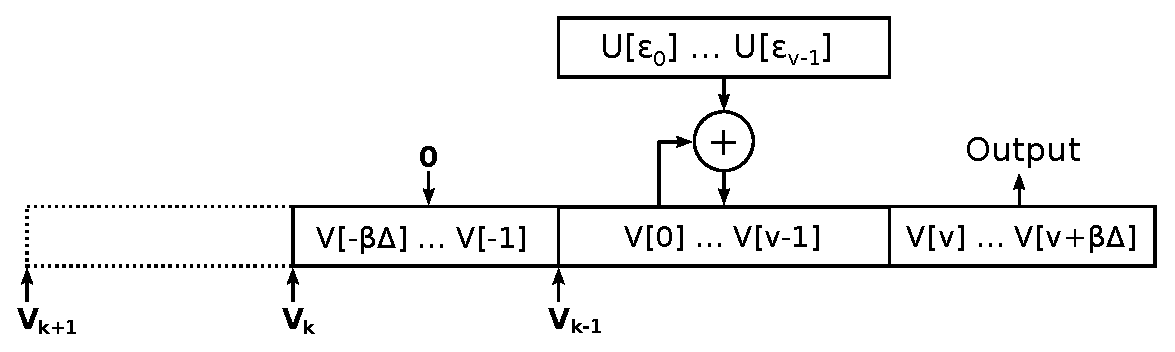
\includegraphics[width=0.99\linewidth]{../source/wbuf_e}
    \caption[W correlation]{Correlation of V}
    \label{fig:wbuf}
\end{figure}

Fig.~\ref{fig:wbuf} shows the output correlator, another view of buffer V.
The output stream flows from left to right,
being initialized to 0 outside the accumulation region.
After $U_\epsilon$ is added to V, the $V_0$ index moves $H_V$ points
to the left, leaving $H_V$ newly minted output points.

Elements of V are accumulated squares of magnitudes.
An attempt was made to accumulate vectors,
with the idea that the phase rotations might sync up,
but it didn't work in simulation.
So, angle data from the FFT is discarded.
